
\section{Proposed methods}

\begin{frame}[plain]
   \sectionpage
\end{frame}

\frame{
   \frametitle{From the literature}

   \textbf{\citet{mankowska2014}}
   \begin{itemize}
      \item MIP model
      \item VNS-based meta-heuristic (deterministic moves)
   \end{itemize}

   \vspace*{18pt}

   \textbf{\citet{lasfargeas2019}}
   \begin{itemize}
      \item Several variations of a constructive heuristic
      \item VNS-based meta-heuristic (randomized moves)
   \end{itemize}
}

\frame{
   \frametitle{MIP-based methods}

   \textbf{Lower bounds with CPLEX}
   \begin{itemize}
      \item In \citet{mankowska2014}, CPLEX 12.3 --- June, 2011
      \item Our experiment: CPLEX 20.1 --- December, 2020
      \begin{itemize}
         \item Pre-processing
         \item Parameter setting
         \item MIP warmstart
      \end{itemize}
   \end{itemize}
}

\frame{
   \frametitle{MIP-based methods}

   \textbf{Fix and optimize matheuristic}
   \begin{itemize}
      \item Model from the literature
      \item Initial solution: constructive heuristic \citep{mankowska2014}
      \item Each iteration: optimizes pair of routes
      \item Stops when the search stales
   \end{itemize}
}

\frame{
   \frametitle{Indirect search methods}

   \textbf{Local search-based methods can be expensive}
   \begin{itemize}
      \item Tricks to reduce work for evaluating some moves
      \item But the synchronization constraints are too impacting
      \begin{itemize}
         \item Clever solution representation \citep{mankowska2014, lasfargeas2019}
         \item Optimized moves, ahead detection of cross-synchronization
      \end{itemize}
   \end{itemize}

   \vspace*{18pt}

   \textbf{Our proposal:} indirect search \citep{drexl2012}
}


\frame{
   \frametitle{Indirect search methods}

   \textbf{BRKGA}
   \begin{itemize}
      \item Main concept by \citet{bean1994}
      \item Most popular version by \citet{gonccalves2011art}
   \end{itemize}

   \vspace*{18pt}

   \textbf{Intensification components}
   \begin{itemize}
      \item Island model (also in \citet{toso2015})
      \item Multi-parent mating
      \item Implicit path relinking on random keys space
      \item Proposed by \citet{andrade2021}
   \end{itemize}
}

\frame{
   \frametitle{Indirect search methods}

   \textbf{For the home health care problem}
   \begin{itemize}
      \item BRKGA $\Rightarrow$ evolves the \emph{task insertion sequence}
      \item The proposed decoder \textbf{embeds} a greedy heuristic
      \item A \emph{best-insertion heuristic decoder} builds a routing solution from the TIS
   \end{itemize}

   \vspace*{12pt}

   \begin{figure}
      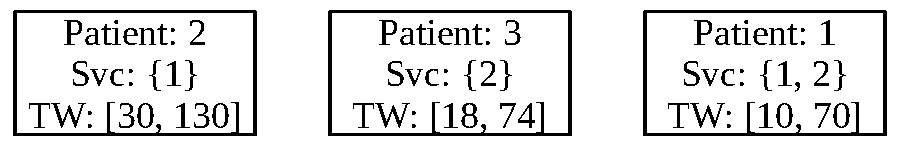
\includegraphics[width=0.5\textwidth]{fig/decoder-tis}
   \end{figure}
}

